\chapter {Analysis on players data}
The previous phases of data cleaning resulted in a dataset of 917 players with 114 votes each.
Analysis are performed on different abstraction levels.
At the beginning, high-level evaluations were made to discover informations on the number of played matches  (mean, min, max etc.). Figure \ref{fig:countMatch} is an exapmle of this analysis: it shows how many players played foreach given number of matches.
\\
\begin{figure}[H]
  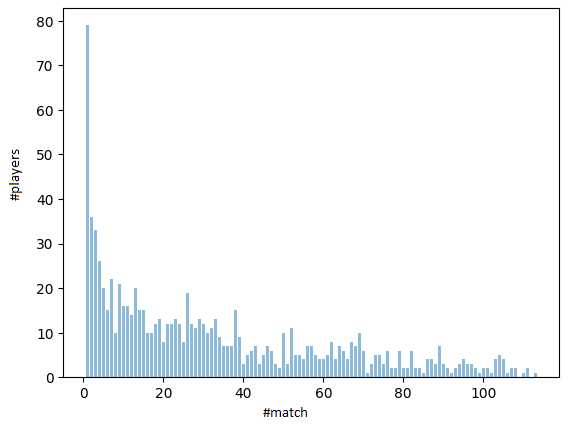
\includegraphics[scale=0.7]{images/img-01.png}
    \centering
   \caption{\textit{Count number of players that played a certain number of matches.}}
  \label{fig:countMatch}
\end{figure}

Similarly, a fine grained analysis has been made by grouping players per role, as shown in figure \ref{fig:countMatchPerRole}, but no relevant differences have been found.
\begin{figure}[h]
  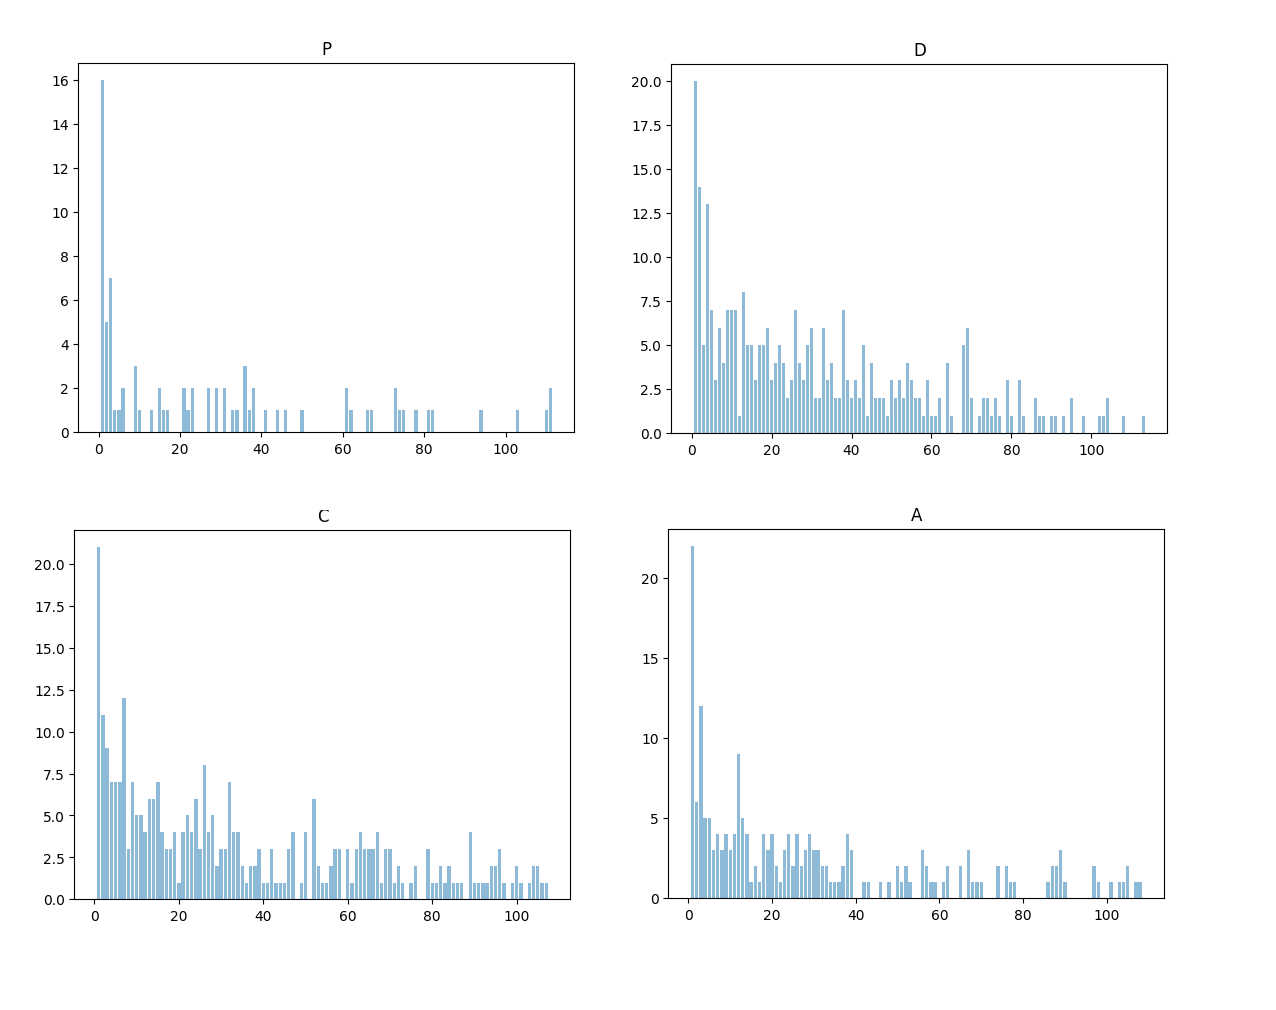
\includegraphics[scale=0.4]{images/img-02.png}
    \centering
   \caption{\textit{Count number of players of such role that played a certain number of matches.
   Legend: P = Goalkeeper, D = Defender, C = Midfielder, A = Striker}}
  \label{fig:countMatchPerRole}
\end{figure}

\begin{figure}[H]
  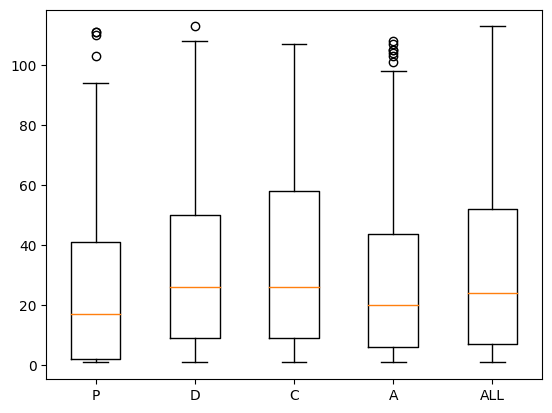
\includegraphics[scale=0.8]{images/quantile.png}
  \centering
   \caption{\textit{Box plot of number of match played. 
   Legend: P = Goalkeeper, D = Defender, C = Midfielder, A = Striker, ALL = All Players}}
  \label{fig:boxPlotMatchPlayed}
\end{figure}


From figure \ref{fig:countMatch},\ref{fig:countMatchPerRole} and \ref{fig:boxPlotMatchPlayed} we can see that most players in the dataset played very few matches. In fact we computed that, on average, 32 matches are played (of the 114 total) and 75\% of the players (almost 687) played less than 52 games. This could lead to some problems because it means that the process of interpolation would have ended up filling a lot values distorting the results of the analysis. In order to solve this issue we decided, for most part of the project, to focus on a subset of players that played at least 100 games .

\section{Data correlation}
The goal is discovering, if present, seasonality on players' votes. In order to achieve such target, \textit{Pearson Correlation Index} has been used.
As mentioned, we have been careful not to consider results biased by the process of interpolation: if we look at figure \ref{fig:box_plot_pearson} we can see that considering players with a lot of interpolated votes (small number of match played) we get best pearsons coefficients that seem very high but this is due to the lack of real values; looking at player that played more matches we can in fact say that no relevant seasonality can be detected.
\begin{figure}[h]
  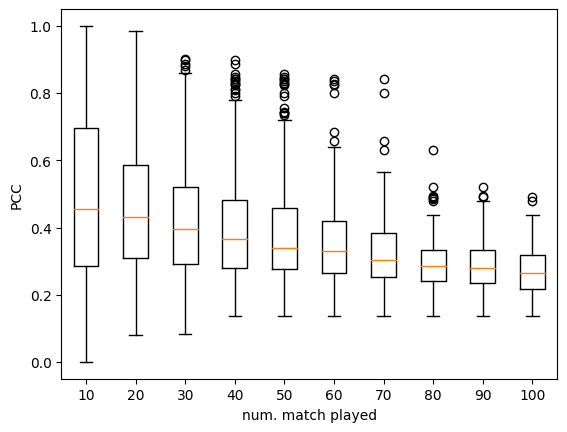
\includegraphics[scale=0.75]{images/quantile_pcc.png}
  \centering
   \caption{\textit{Box plots of the best perason correlation coefficients computed on fantavoti of players that played at least the number of matches in the x axis.}}
  \label{fig:box_plot_pearson}
\end{figure}

Figure \ref{fig:playereg} reports pearson coefficient computed on an example player for voti, fantavoti and bonus.

\begin{figure}[H]
  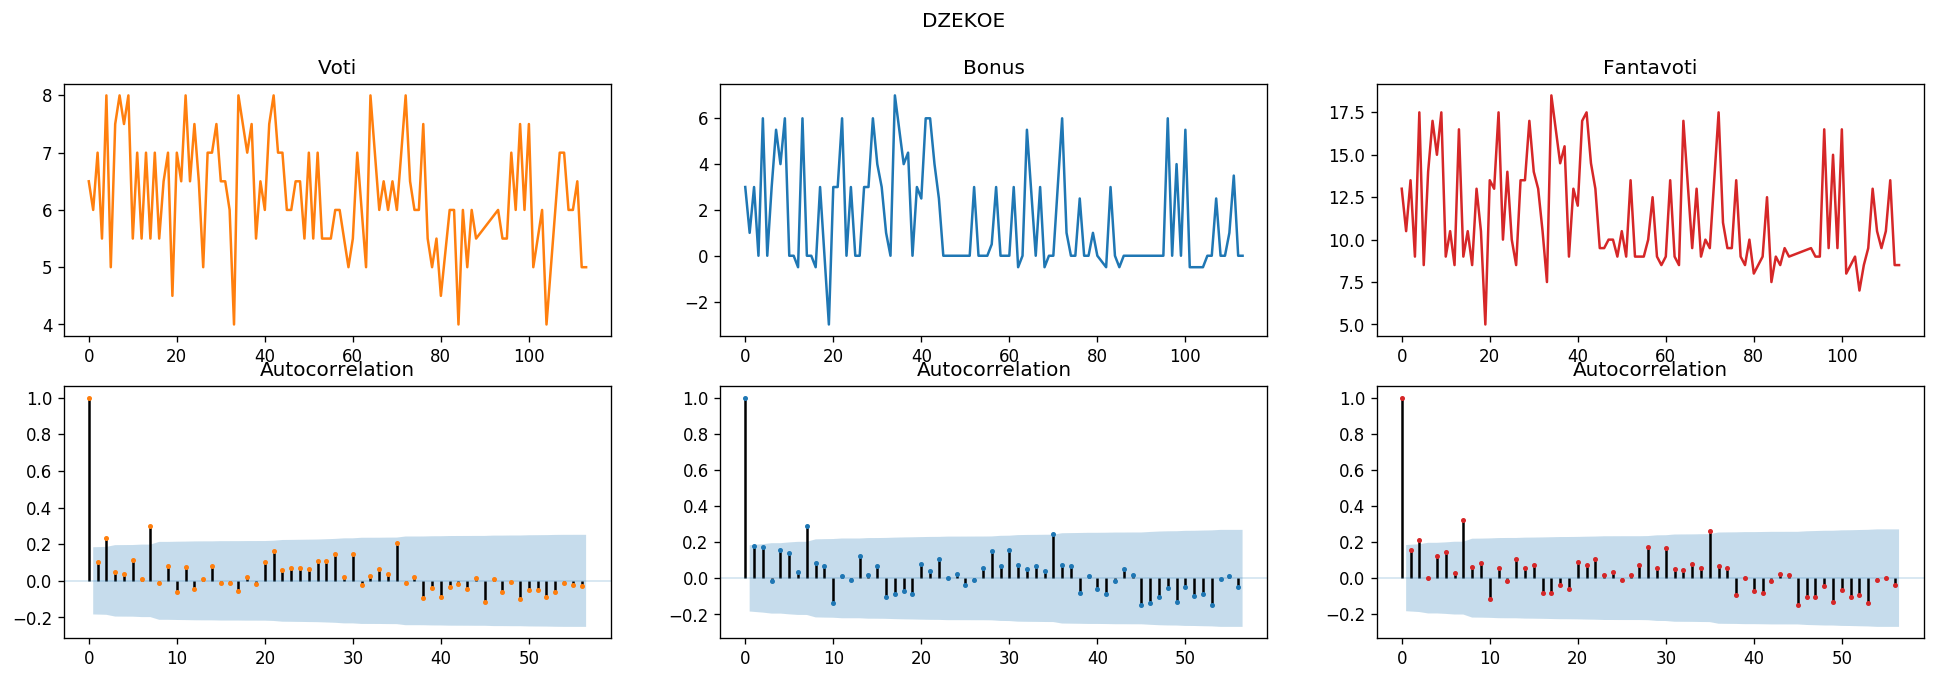
\includegraphics[width=\textwidth]{images/dzeko_all_infos.png}
   \caption{\textit{The image shows storic series and respective Pearson correlations for ''Edin Dzeko''.}}
  \label{fig:playereg}
\end{figure}

\section{Normality test}
Normalty test has been used on votes and fantavotes both in order to determine if the two datasets could be modeled similarly to a normal distribution.
QQ-plot and histograms of votes showed a correlation between votes and normal distribution for almost all players (Figure \ref{fig:hist_votes} and Figure \ref{fig:qqplot_votes}).
The same can't be asserted about fantavotes (Figure \ref{fig:hist_fantavotes} and Figure \ref{fig:qqplot_fantavotes}).

\begin{figure}[H]
  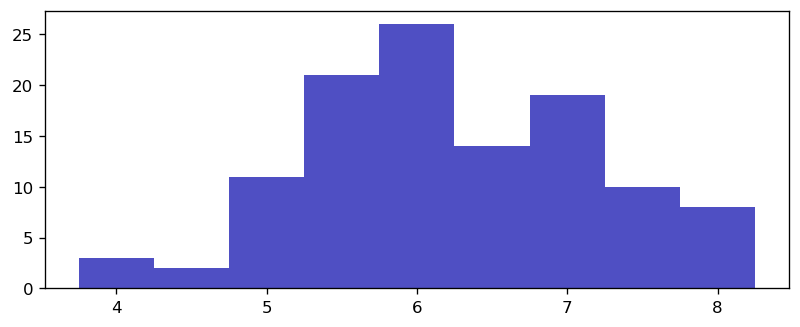
\includegraphics[scale=0.5]{images/dzeko_normality_test_voti_barchart.png}
    \centering  
   \caption{\textit{'Votes' histogram for ''Edin Dzeko''.}}
  \label{fig:hist_votes}
\end{figure}

\begin{figure}[H]
  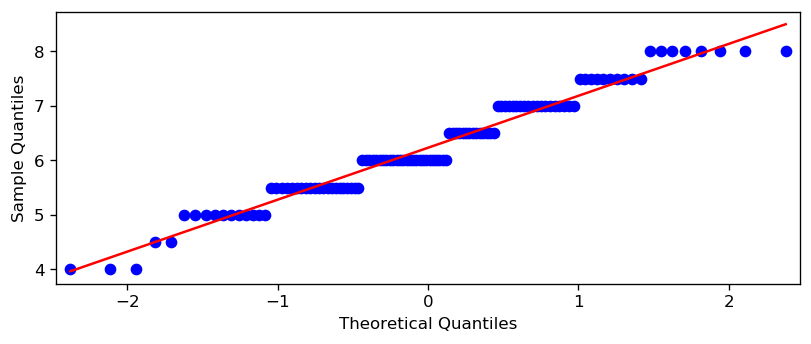
\includegraphics[scale=0.5]{images/dzeko_normality_test_voti_qqplot.png}
   \centering  
   \caption{\textit{'Votes' qqplot for ''Edin Dzeko''.}}
  \label{fig:qqplot_votes}
\end{figure}

\begin{figure}[H]
  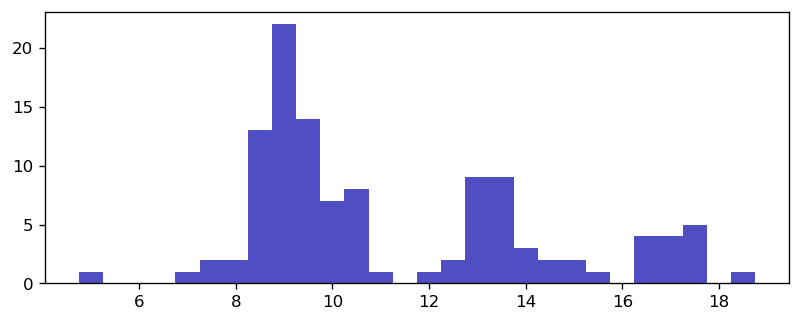
\includegraphics[scale=0.5]{images/dzeko_normality_test_fantavoti_barchart.png}
   \centering  
   \caption{\textit{'Fantavotes' histogram for ''Edin Dzeko''.}}
  \label{fig:hist_fantavotes}
\end{figure}

\begin{figure}[H]
  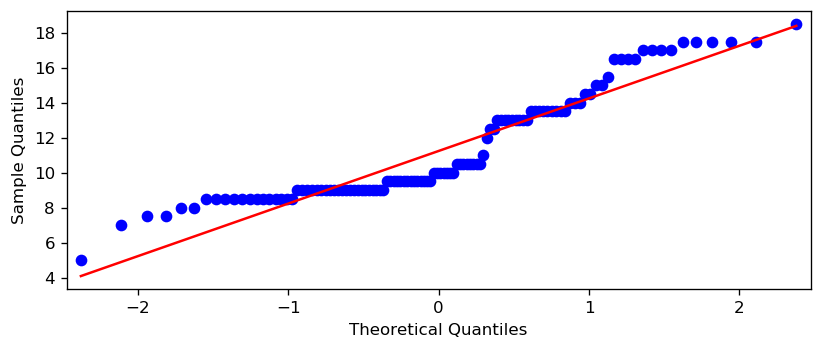
\includegraphics[scale=0.5]{images/dzeko_normality_test_fantavoti_qqplot.png}
   \centering  
   \caption{\textit{'Fantavotes' qqplot for ''Edin Dzeko''.}}
  \label{fig:qqplot_fantavotes}
\end{figure}






  